\documentclass{beamer}

\mode<presentation> {
  \usetheme{CambridgeUS}
  \setbeamercovered{transparent}
}

\usepackage[english]{babel}
\usepackage[utf8]{inputenc}
\usepackage{times}
\usepackage[T1]{fontenc}
\usepackage{fontawesome}
\usepackage[backend=biber, style=numeric]{biblatex}
\addbibresource{SeminarTalk.bib}

\title[Wildlife Tracking with IoT]{Using Internet of Things (IoT) Networks for Wildlife Tracking}
\author{Collin Beane}
\institute[U of Minn, Morris]
{
  Division of Science and Mathematics \\
  University of Minnesota, Morris \\
  Morris, Minnesota, USA
}
\date{\today}

\begin{document}

\begin{frame}
  \titlepage
\end{frame}

\begin{frame}
  \frametitle{Hypothetical Scenario}
  \begin{figure}[htbp]
    \centering
    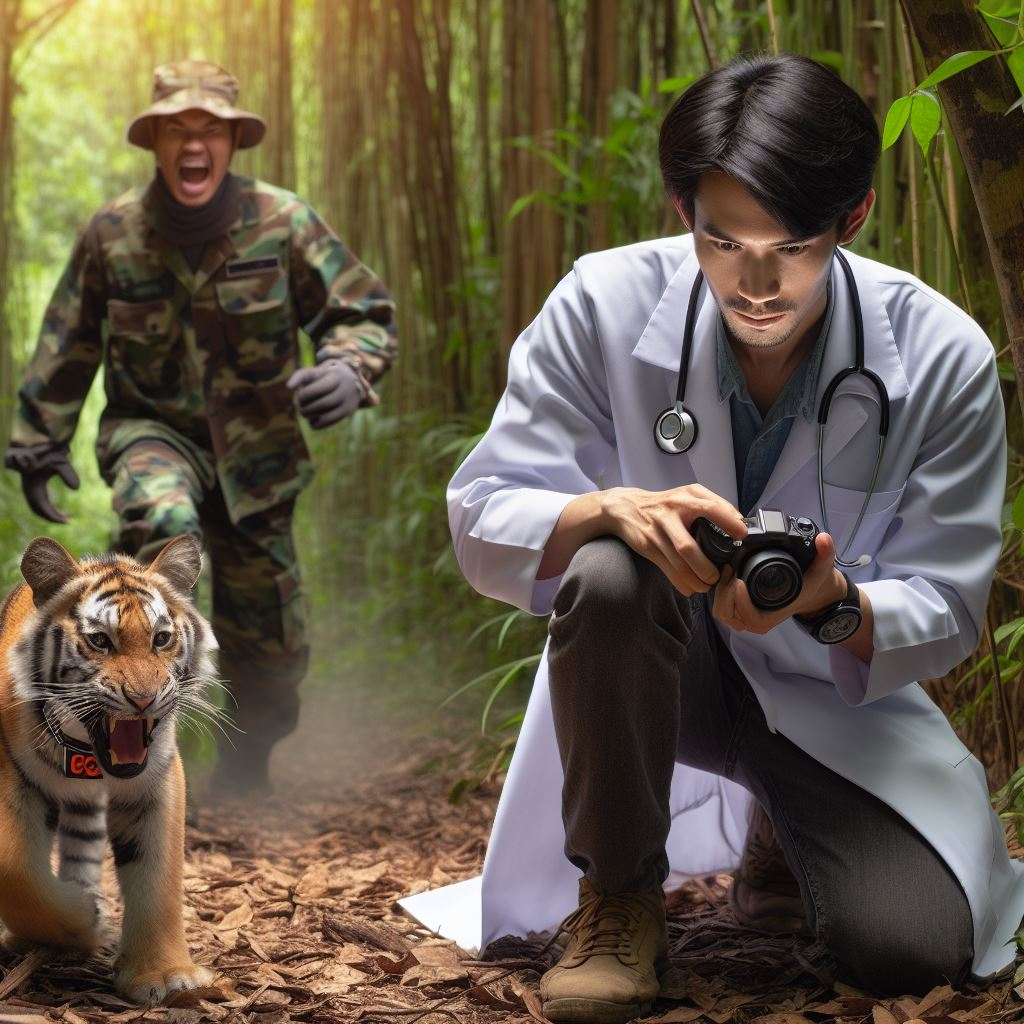
\includegraphics[height=.8\textheight]{Biologging_scenario.jpg}
    \label{fig:Hypothetical_biologging}
  \end{figure}
\end{frame}


\begin{frame}
  \frametitle{Outline}
  \tableofcontents[sectionstyle=show,subsectionstyle=hide]
\end{frame}

% Section and subsections will appear in the presentation overview and table of contents.

\section{Background}

\subsection{What is Biologging?}
\begin{frame}{Background}
  \frametitle{Introduction to Biologging}
        \begin{figure}[htbp]
          \centering
          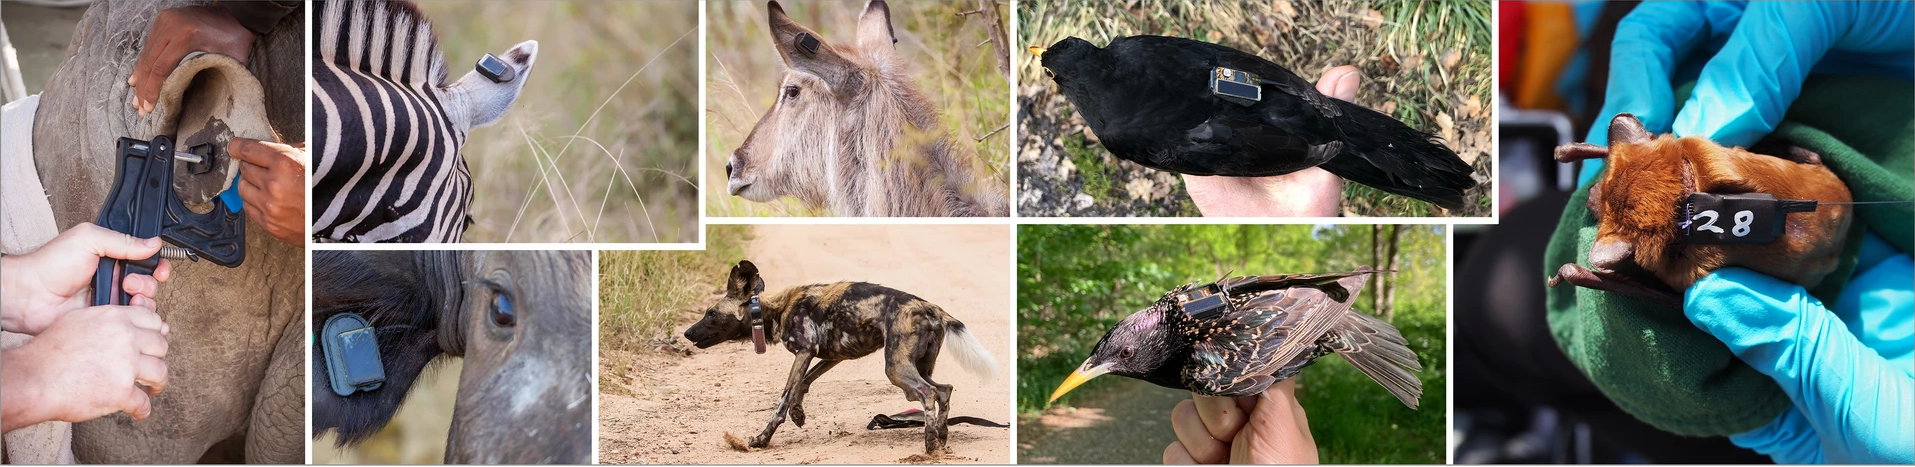
\includegraphics[width=.75\textwidth, height=.2\textheight]{TrakingDevices.png}
          \caption{Animals With SigFox enabled biologging tags \cite{wild2023multi}}
          \label{fig:TaggedAnimals}
        \end{figure}
        \begin{itemize}
          \item \textbf{Definition:} "Investigation of phenomena in or around free-ranging organisms beyond human visibility or experience \cite{boyd2004bio}"
          \item \textbf{Method:} Tracking wild animals using electronic devices attached to animals
          \item $\uparrow$ Popularity in early 2000s, practiced since 60's
          \item Pivotal role in understanding animal behavior and ecology
        \end{itemize}
\end{frame}

\begin{frame}{Background}
  \frametitle{Applications of Biologging}
  \begin{columns}
    \begin{column}{0.5\textwidth}
  \begin{figure}[htbp]
    \centering
    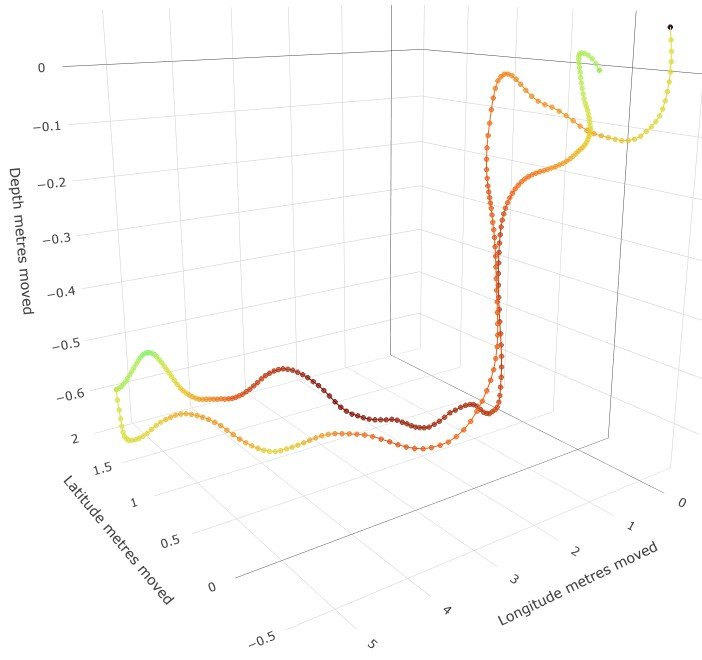
\includegraphics[width=\textwidth]{prairie_dog_map.jpg}
    \caption{3D movement of a prairie dog \cite{Kidangoor_2024}}
    \label{fig:prairie_dog_3D_movement}
  \end{figure}
\end{column}
\begin{column}{0.5\textwidth}
  \begin{figure}[htbp]
    \centering
    
\includegraphics[width=.5\textwidth]{prairie_dog.jpg}
    \label{fig:prairie_dog}
  \end{figure}
  \begin{itemize}
    \item Track animal movements, behaviors, and migration patterns
    \item Collect data on the animal's environment.
  \end{itemize}
\end{column}
\end{columns}
\end{frame}

\begin{frame}{Background}
  \frametitle{Impact and Importance}
        \begin{itemize}
          \item Insights into organisms in hostile or hard-to-reach environments
          \item Study previously inaccessible aspects of animal life
          \item Inform conservation efforts and protect endangered species
          \item Tool for general data collection
        \end{itemize}
\end{frame}

\begin{frame}{Background}
  \frametitle{Other Biologging Methods}
  \begin{columns}
    \begin{column}{0.5\textwidth}
        \begin{itemize}
          \item Cellular networks; High Cost
          \begin{itemize}
            \item \$250/device
            \item 10\textcent/message
          \end{itemize}
          \item Radio Frequency (5-1000m)
          \begin{itemize}
            \item Periodic tracking records
            \item Time stamped data
          \end{itemize}
        \end{itemize}
      \end{column}
      \begin{column}{.5\textwidth}
        \begin{figure}[htbp]
          \centering
          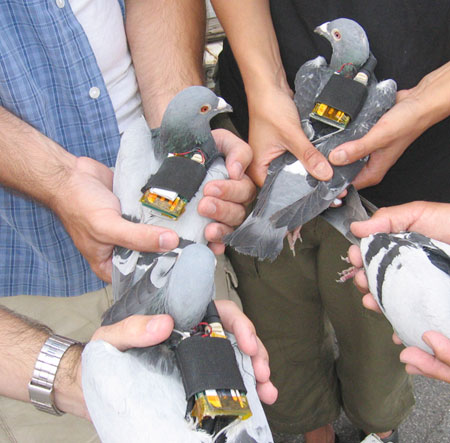
\includegraphics[width=\textwidth]{PigeonCellular.jpg}
          \caption{Pigeons Equipped with cellular trackers \cite{Martin_2006}}
          \label{fig:PigeonCellular}
        \end{figure}
      \end{column}
    \end{columns}
\end{frame}

\subsection{Wireless Networks Basics}

\begin{frame}{Background}
  \frametitle{Data Transmission}
  \begin{columns}
    \begin{column}{0.4\textwidth}
        \begin{figure}[htbp]
          \centering
          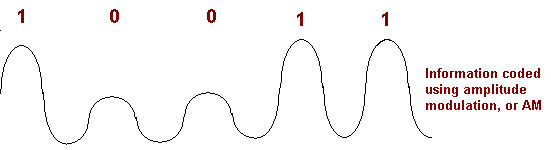
\includegraphics[width=\textwidth]{AMdataTransmission.jpg}
          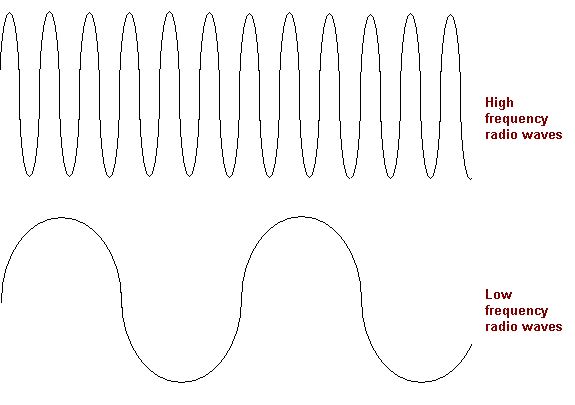
\includegraphics[width=.8\textwidth]{Frequency_graph.png}
          \caption{Data representation using amplitude modulation and frequency \cite{AMdata}}
          \label{fig:AM_data_transmission}
        \end{figure}
    \end{column}
    \begin{column}{0.6\textwidth}
      \begin{itemize}
        \item Data encoded into 1's and 0's
          \begin{itemize}
            \item Represented by amplitude
            \item More complex methods are used
          \end{itemize}
        \item Frequency determines data rate and range
        \begin{itemize}
          \item higher freq $\implies$ higher data-rate
          \item higher freq $\implies$ lower range
        \end{itemize}
        \item Received and translated by other devices
      \end{itemize}
    \end{column}
  \end{columns}
\end{frame}

\begin{frame}{Background}
  \frametitle{Wireless Network Frequencies and Range}
  \begin{columns}
    \begin{column}{0.5\textwidth}
      \begin{itemize}
        \item WLAN frequencies
          \begin{itemize}
            \item 2.4GHz/5GHz/6GHz
            \item Range $\approx$ 200m (2.4Ghz)
          \end{itemize}
        \item LPWAN Frequencies
          \begin{itemize}
            \item $<$1GHz (depends on region)
            \item Range $\approx$ 20-40km
          \end{itemize}
      \end{itemize}
    \end{column}
    \begin{column}{0.5\textwidth}
      \begin{figure}[htbp]
        \centering
        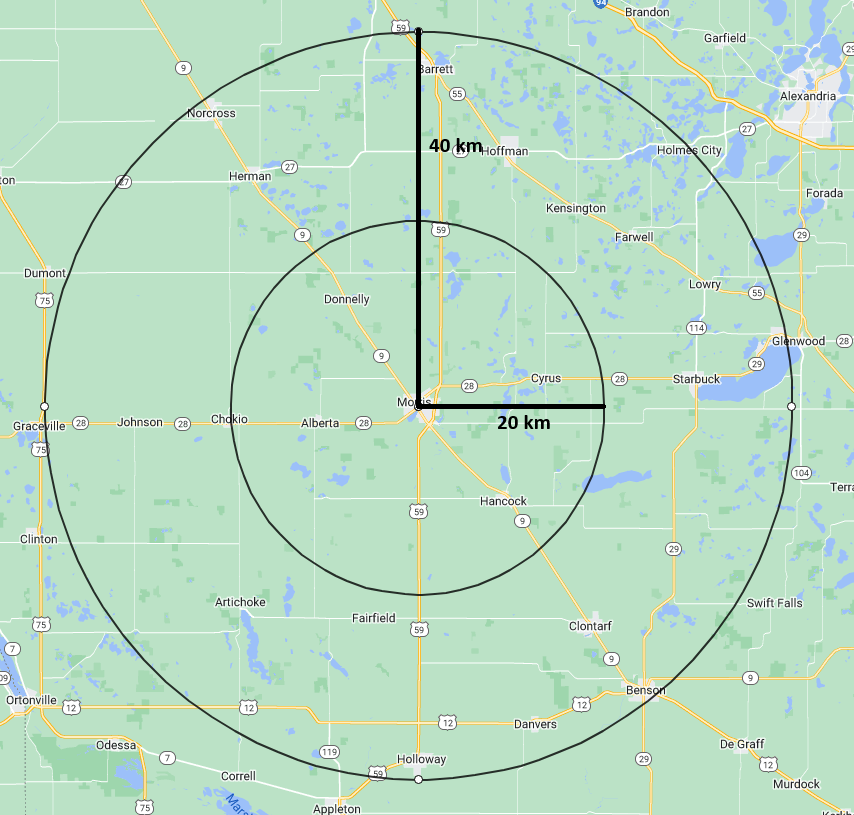
\includegraphics[width=.9\textwidth]{Range_comparisons.png}
        \caption{200m, 20km, and 40km radius around Morris, MN}
        \label{fig:Range_map}
      \end{figure}
  \end{column}
  \end{columns}
\end{frame}

\begin{frame}{Background}
  \frametitle{Frequency Hopping and Modulation}
  \begin{columns}
    \begin{column}{0.5\textwidth}
      \begin{figure}[htbp]
        \centering
        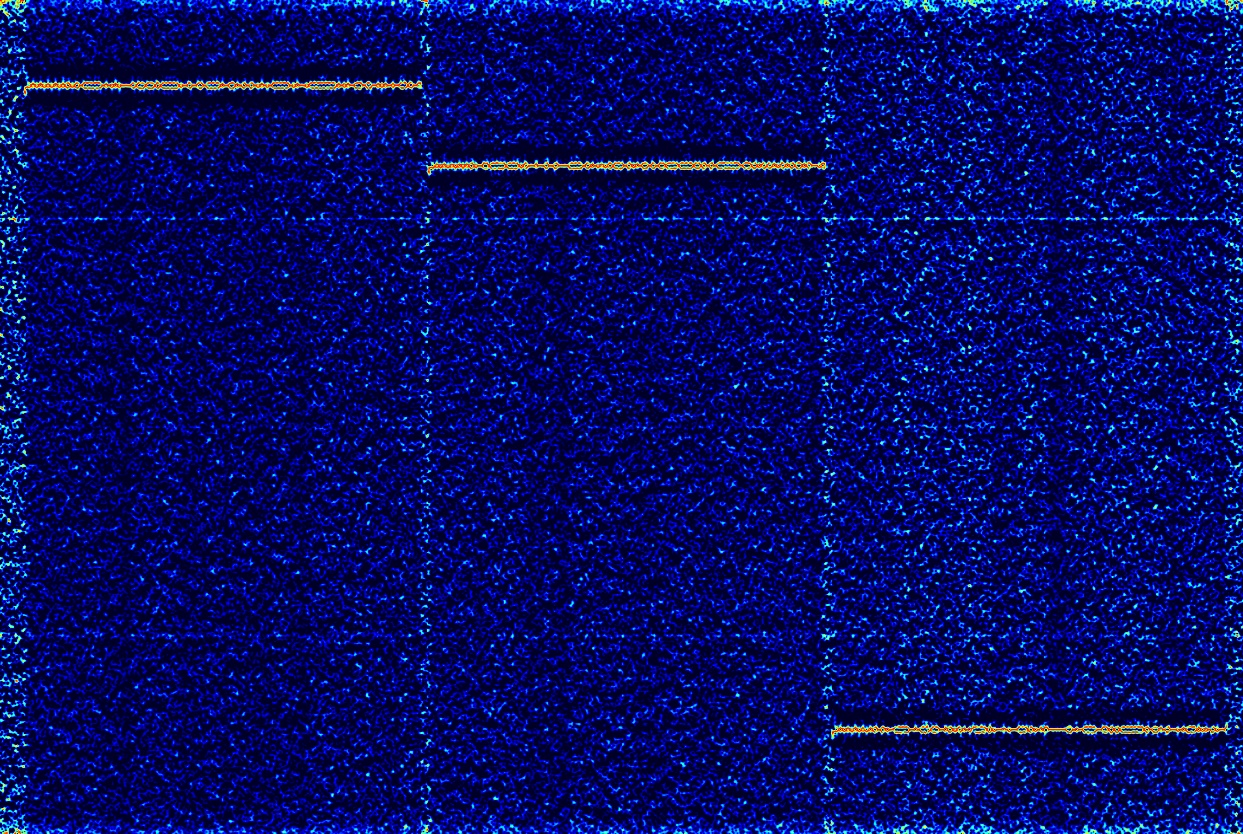
\includegraphics[width=.7\textwidth]{Sigfox_Spectrum_Analysis.jpg}
        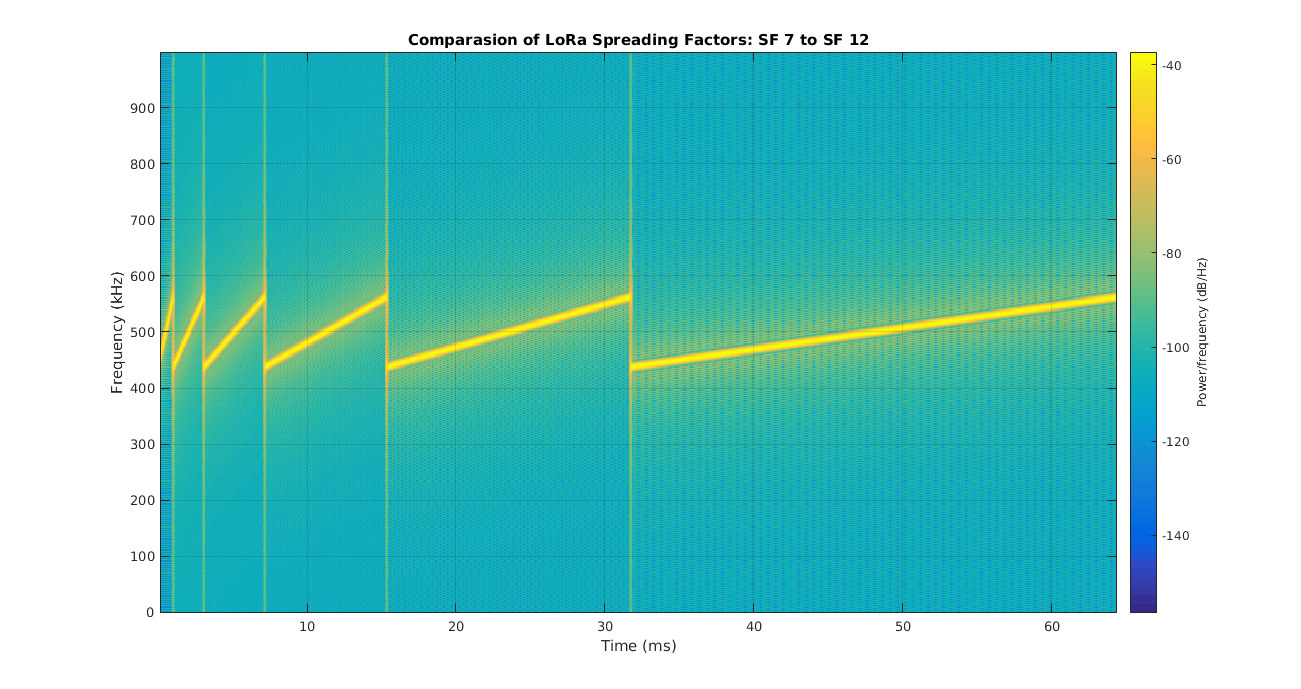
\includegraphics[width=.9\textwidth]{Chirp.png}
        \caption{CHRIP and frequency hopping modulation}
        \label{fig:Frequency_hopping_and_modulation}
      \end{figure}
  \end{column}
    \begin{column}{0.5\textwidth}
      \begin{itemize}
        \item Resistance to interference
        \item Ensures delivery
        \item Frequency hopping
          \begin{itemize}
            \item Transmits message 3 times
            \item Pseudo randomly hops to new frequency
          \end{itemize}
        \item CHIRP (Compressed High Intensity Radar Pulse) spread spectrum
          \begin{itemize}
            \item Gradually raises/lowers frequencies
            \item $\uparrow$ SF $\Rightarrow$ $\downarrow$ modulation rates
          \end{itemize}
      \end{itemize}
    \end{column}
  \end{columns}
\end{frame}


\subsection{What is the Internet of Things?}

\begin{frame}{Background}
  \frametitle{What is the Internet of Things?}
  \begin{itemize}
    \item \textbf{Empowering physical objects with sensors and software for autonomous interaction}
    \item Can either connect via wired or wireless connection
    \item Many applications: Healthcare, agriculture, and of course conservation
  \end{itemize}
\end{frame}

\begin{frame}{Background}
  \frametitle{Layers of an IoT System}
  \begin{columns}
    \begin{column}{0.6\textwidth}
      \begin{itemize}
        \item Application Layer
          \begin{itemize}
            \item Processes and uses data
          \end{itemize}
        \item Network Layer
          \begin{itemize}
            \item Establishes connection to internet and IoT devices
            \item Transmits data to and from the other layers
          \end{itemize}
        \item Perception Layer
          \begin{itemize}
            \item Collects data from the environment or...
            \item Interacts with the physical device
          \end{itemize}
      \end{itemize}
    \end{column}
    \begin{column}{0.4\textwidth}
      \begin{figure}[htbp]
        \centering
        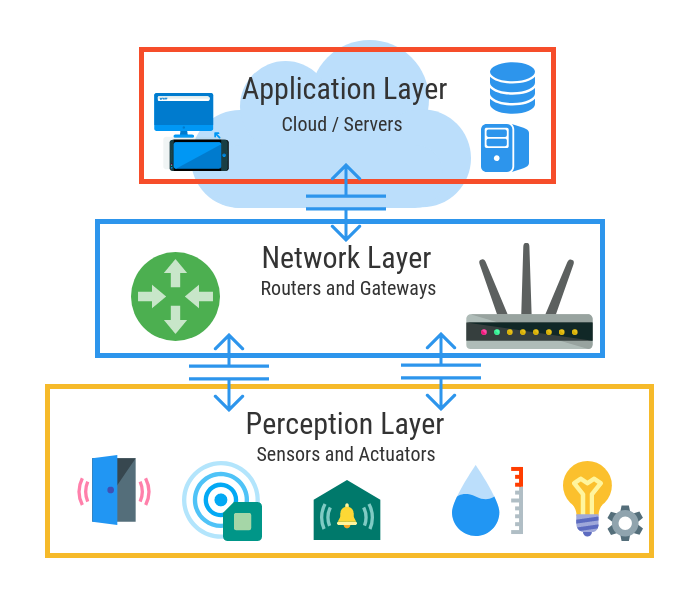
\includegraphics[width=\textwidth]{three-layer-iot-architecture.png}
        \caption{Layer Structure of an IoT System \cite{Calihman_2021}}
        \label{fig:IoT_Layers}
      \end{figure}
  \end{column}
  \end{columns}
\end{frame}



\section{Components of a Modern Biologging System}

\subsection{Sensor Devices}

  \begin{frame}{Components of a Modern Biologging System}
    \frametitle{Sensor Devices (tags)}
    \begin{columns}
      \begin{column}{.5\textwidth}
        \begin{itemize}
          \item IoT perception layer 
          \item Required Components
          \begin{itemize}
            \item Antenna
            \item Microcontroller
            \item Battery
            \item Sensor(s)
          \end{itemize}
          \item Optional Components
          \begin{itemize}
            \item Solar panel
            \item Extra storage
          \end{itemize}
        \end{itemize}
      \end{column}
      \begin{column}{0.5\textwidth}
        \begin{figure}[htbp]
          \centering
          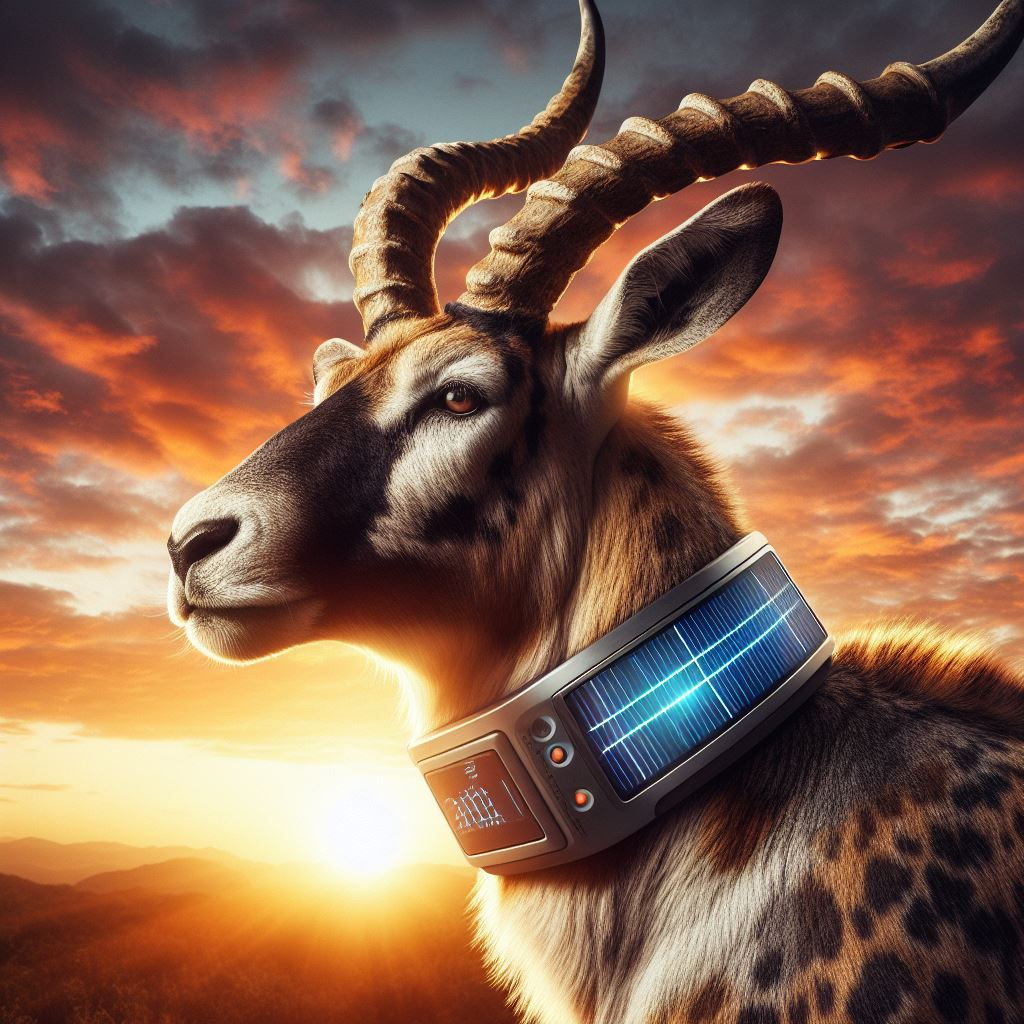
\includegraphics[height=.6\textheight]{Solar_collar.jpg}
          \caption{Animal wearing a solar powered biologging collar, looking majestic [DALL$\cdot$E 3]}
          \label{fig:Solar_collar}
        \end{figure}
    \end{column}
    \end{columns}
  \end{frame}

  \begin{frame}{Components of a Modern Biologging System}
    \frametitle{Sensor Devices}
    \begin{figure}[htbp]
      \centering
      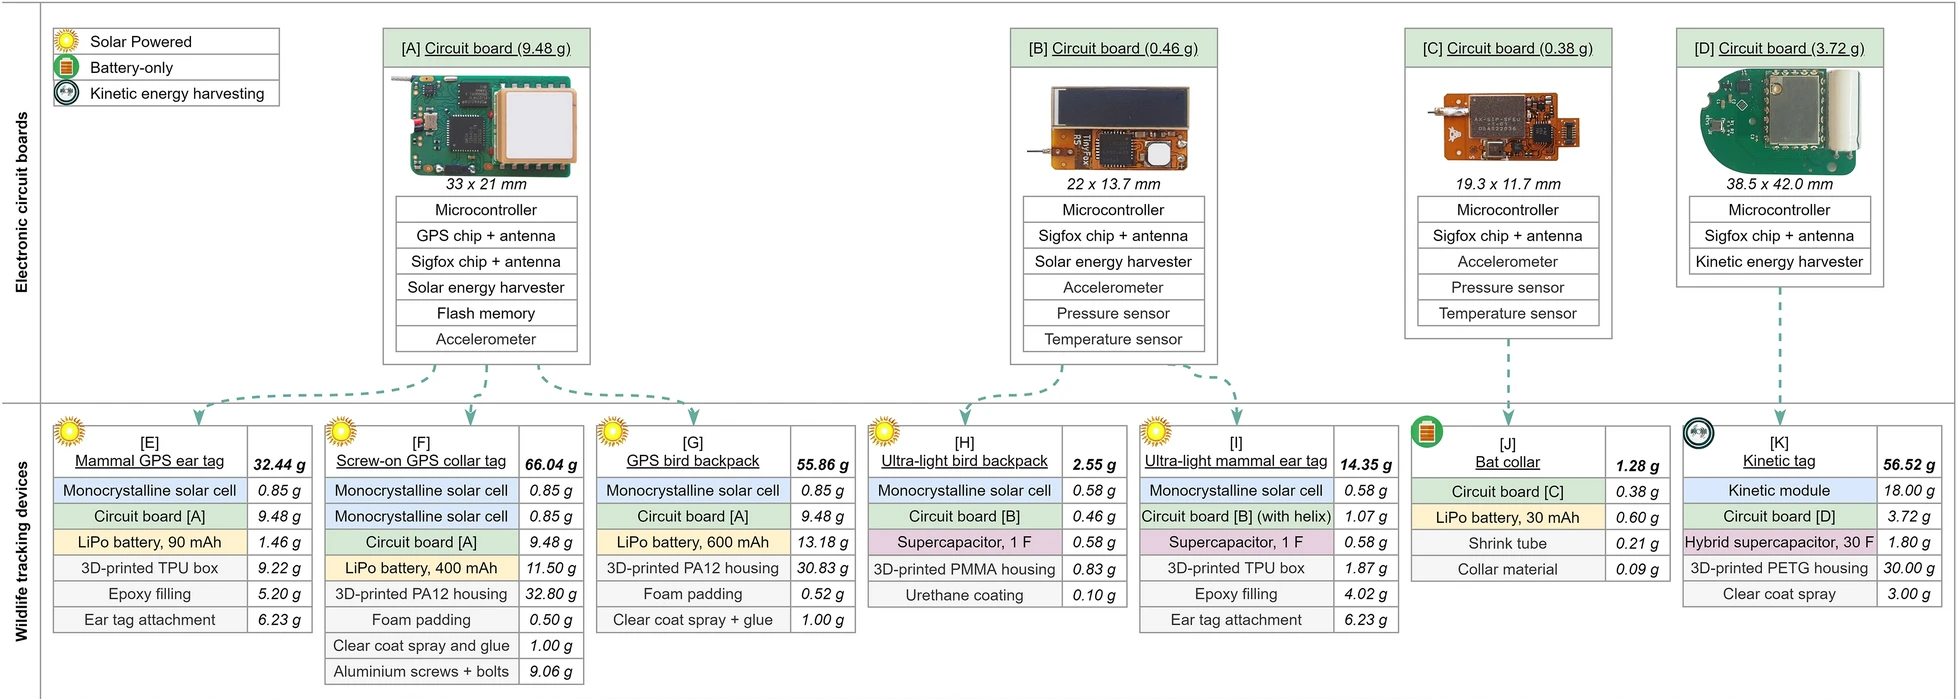
\includegraphics[width=\textwidth]{SigFox_Sensor_device.png}
      \caption{SigFox Biologging Sensor Device \cite{wild2023multi}}
      \label{fig:SigFox_Biologging_device}
    \end{figure}
  \end{frame}

\subsection{Base Stations}

  \begin{frame}{Components of a Modern Biologging System}
    \frametitle{Base Stations}
    \begin{columns}
      \begin{column}{0.4\textwidth}
        \begin{figure}[htbp]
          \centering
          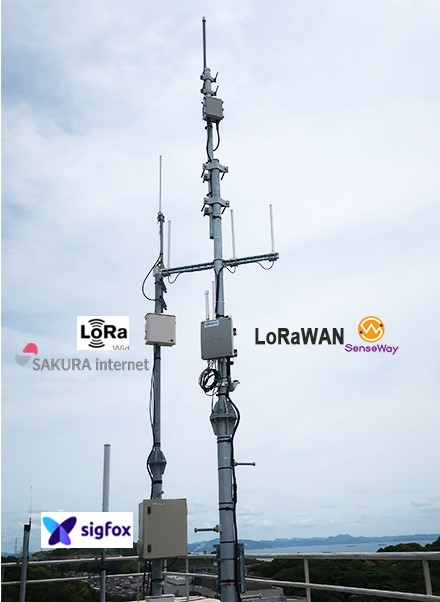
\includegraphics[height=.7\textheight]{BaseStation.jpg}
          \caption{YRP hybrid base station \cite{miyajima_2020}}
          \label{fig:LPWAN_Base_Station}
        \end{figure}
      \end{column}
      \begin{column}{0.6\textwidth}
        \begin{itemize}
          \item IoT network layer
          \item Components
          \begin{itemize}
            \item RF receiver and transmitter
            \item Data forwarding engine
            \item Power source
            \item Connection to internet or \ldots
            \item Local Storage
          \end{itemize}
        \end{itemize}
      \end{column}
    \end{columns}
  \end{frame}

\section{Networks for a Biologging System}

\subsection{Networking Outline}
  \begin{frame}{Networking}
    \frametitle{Networking Outline}
    \begin{itemize}
      \item Importance of a Strong Network for Biologging
      \item LPWAN Networks
      \begin{itemize}
        \item SigFox
        \item LoRa
      \end{itemize}
      \item WLAN Networks
      \item Security of LPWAN and WLAN Networks
      \item Which Network is Best for Biologging?
    \end{itemize}
  \end{frame}


\subsection{Importance of a Strong Network}
  \begin{frame}{Networking}
    \frametitle{Importance of a Strong Network for Biologging}
    \begin{columns}
      \begin{column}{0.5\textwidth}
        \begin{itemize}
          \item Safe and secure transmission
          \begin{itemize}
            \item Poachers
          \end{itemize}
          \item Efficient transmission
          \begin{itemize}
            \item Battery life
          \end{itemize}
          \item Easy access to data
          \begin{itemize}
            \item Cloud access
          \end{itemize}
        \end{itemize}
      \end{column}
      \begin{column}{0.5\textwidth}
        \begin{figure}[htbp]
          \centering
          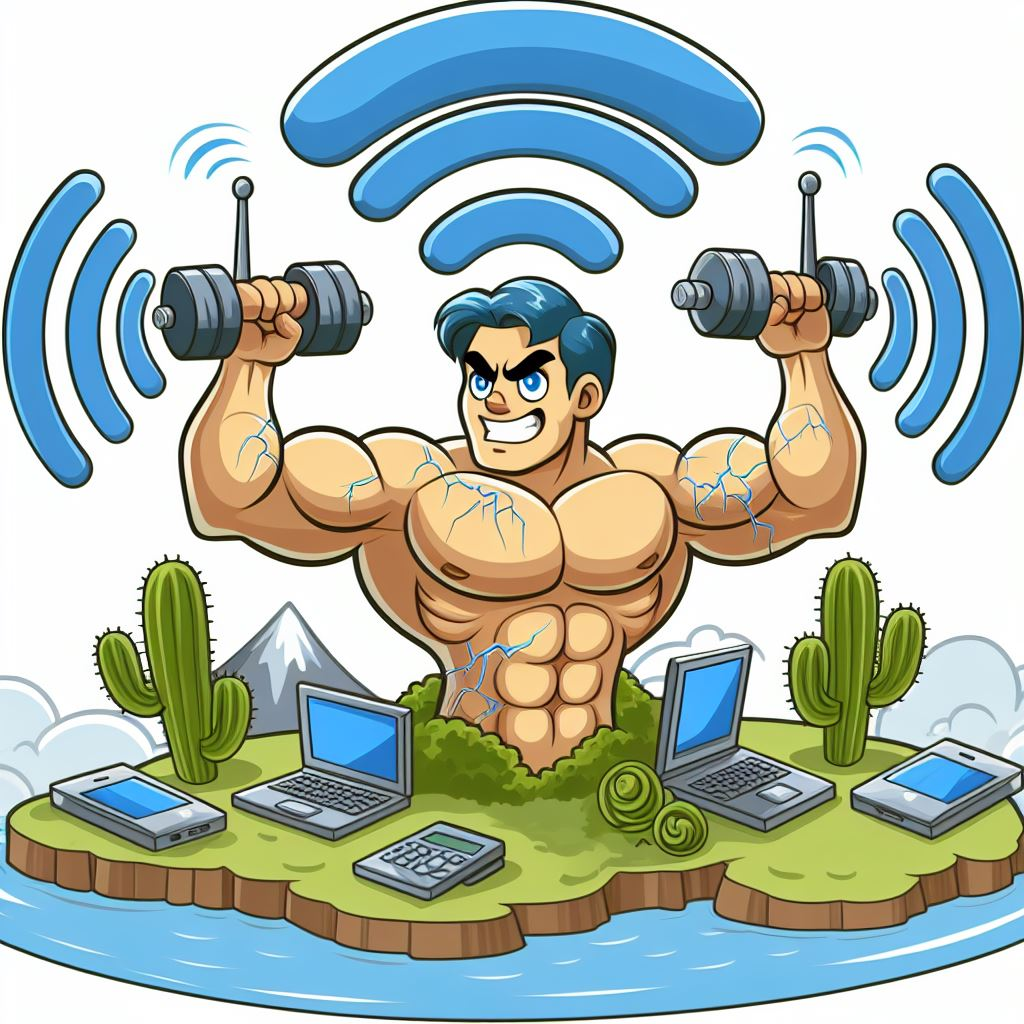
\includegraphics[width=.9\textwidth]{StrongNetwork.jpg}
          \caption{Cartoon depiction of a strong wireless network [DALL$\cdot$E 3]}
          \label{fig:Strong_wireless_network}
        \end{figure}
      \end{column}
    \end{columns}
  \end{frame}

\subsection{LPWAN Networks}

  \begin{frame}{Networking}
    \frametitle{LPWAN Overview}
    \begin{columns}
      \begin{column}{0.4\textwidth}
        \begin{figure}[htbp]
          \centering
          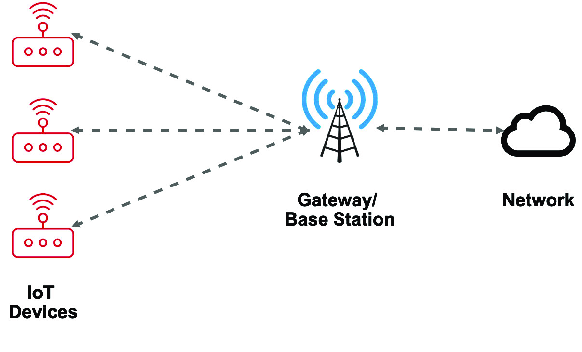
\includegraphics[width=\textwidth]{LPWAN-technologies-network-architecture.png}
          \caption{LPWAN technologies network architecture \cite{LoRaNetworkFernandez}}
          \label{fig:LPWAN_Network_architecture}
        \end{figure}
      \end{column}
      \begin{column}{0.6\textwidth}
        \begin{itemize}
          \item \textbf{L}ow \textbf{P}ower \textbf{W}ide \textbf{A}rea \textbf{N}etwork
          \item Uses unlicensed industrial, scientific and medical radio frequencies (ISM)
          \item 433MHz-928MHz Depending on region (U.S. 915MHz)
          \item Low power consumption
          \item Long range (40km+)
        \end{itemize}
      \end{column}
    \end{columns}
  \end{frame}

  \begin{frame}{Networking}
    \frametitle{SigFox LPWAN}
    \begin{columns}
      \begin{column}{0.5\textwidth}
        \begin{figure}[htbp]
          \centering
          
\includegraphics[width=\textwidth]{sigfox_logo.png}
          \caption{SigFox Logo}
          \label{fig:SigFox_logo}
        \end{figure}
      \end{column}
      \begin{column}{0.5\textwidth}
        \begin{itemize}
          \item Owns and operates global network
          \item Began operation in 2010
          \item Proprietary service
          \item Subscription based service
        \end{itemize}
      \end{column}
    \end{columns}
  \end{frame}


  \begin{frame}{Networking}
    \frametitle{SigFox LPWAN Capabilities}
    \begin{columns}
      \begin{column}{0.5\textwidth}
        \begin{itemize}
          \item 140 messages/day (12 bytes each)
          \item Up to 100bps
          \item 40km+ of range depending on environment
          \item SigFox Atlas for estimating location
          \item 6.5yr battery life w/ 2 AAA batteries (more with solar panel)
        \end{itemize}
      \end{column}
      \begin{column}{0.5\textwidth}
        \begin{figure}[htbp]
          \centering
          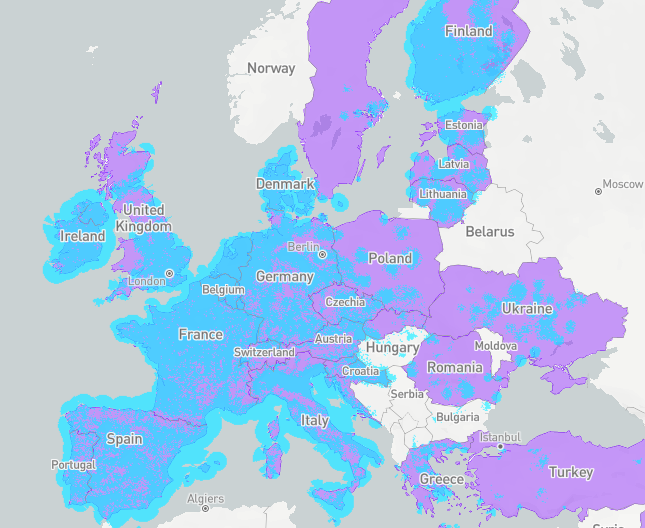
\includegraphics[width=\textwidth]{SigFoxCoverage.png}
          \caption{SigFox Europe Coverage, blue=live coverage, purple=roll-out \cite{Sigfox_0G_Technology_2024}}
          \label{fig:SigFox_Coverage}
        \end{figure}
      \end{column}
    \end{columns}
  \end{frame}

  \begin{frame}{Networking}
    \frametitle{SigFox Operation}
    \begin{columns}
      \begin{column}{0.5\textwidth}
        \begin{figure}[htbp]
          \centering
          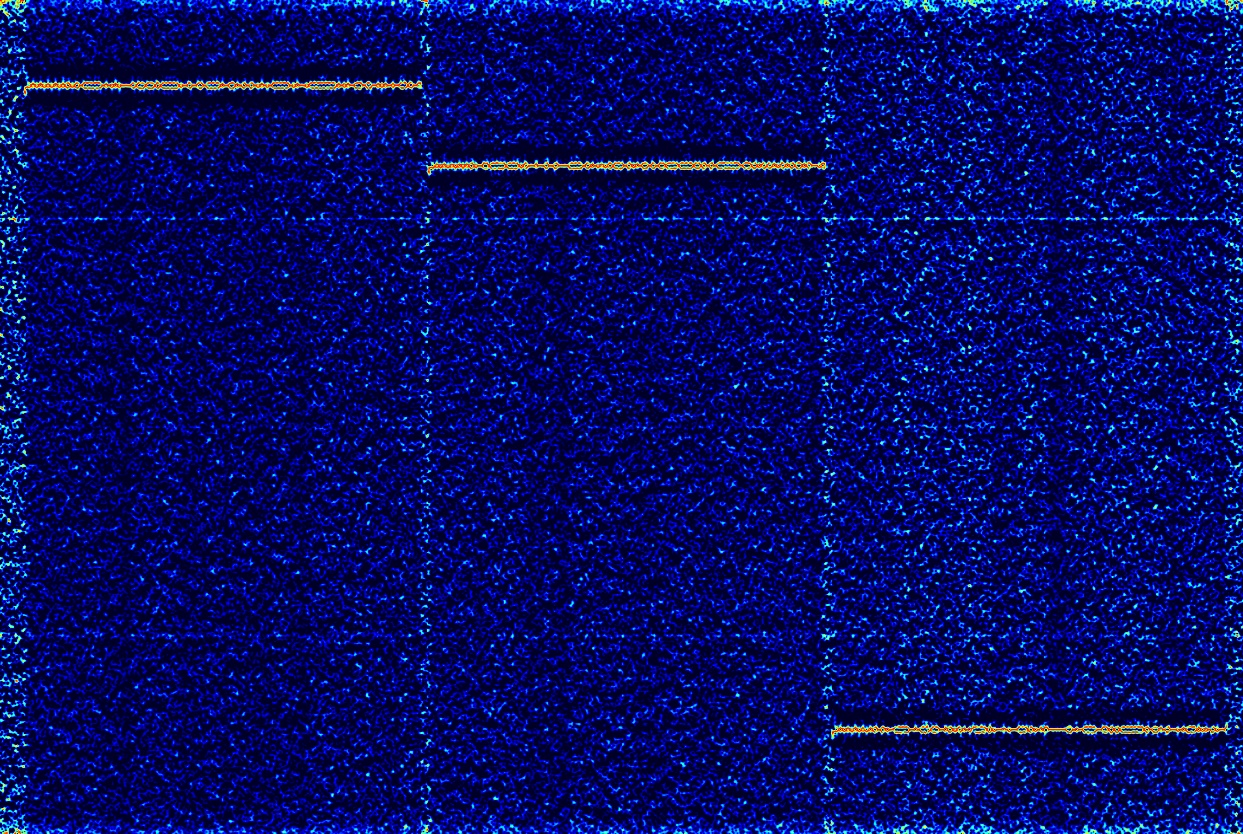
\includegraphics[width=\textwidth]{Sigfox_Spectrum_Analysis.jpg}
          \caption{SigFox frequency hopping modulation \cite{SIGFOXsignalwiki}}
          \label{fig:SigFox_Spectrum}
        \end{figure}
      \end{column}
      \begin{column}{0.5\textwidth}
        \begin{itemize}
          \item Transmission modulation
          \begin{itemize}
            \item Frequency hopping
          \end{itemize}
          \item Proprietary base stations
          \item Devices certification
        \end{itemize}
      \end{column}
    \end{columns}
  \end{frame}

  \begin{frame}{Networking}
    \frametitle{LoRaWAN LPWAN}
    \begin{columns}
      \begin{column}{0.5\textwidth}
        \begin{figure}[htbp]
          \centering
          
\includegraphics[width=\textwidth]{lora_logo.png}
          \caption{LoRa Logo}
          \label{fig:LoRa_logo}
        \end{figure}
      \end{column}
      \begin{column}{0.5\textwidth}
        \begin{itemize}
          \item Standards based system
          \item Public networks available
          \item Self deployable networks
          \item Open source implementations
        \end{itemize}
      \end{column}
    \end{columns}
  \end{frame}

  \begin{frame}{Networking}
    \frametitle{LoRaWAN Operation and Capabilities}
    \begin{columns}
      \begin{column}{0.5\textwidth}
        \begin{itemize}
          \item Unlimited messages/day
          \item CHIRP Spread Spectrum modulation
          \item 20km+ of range depending on environment
          \item Up to 50kbps
        \end{itemize}
      \end{column}
      \begin{column}{0.5\textwidth}
        \begin{figure}[htbp]
          \centering
          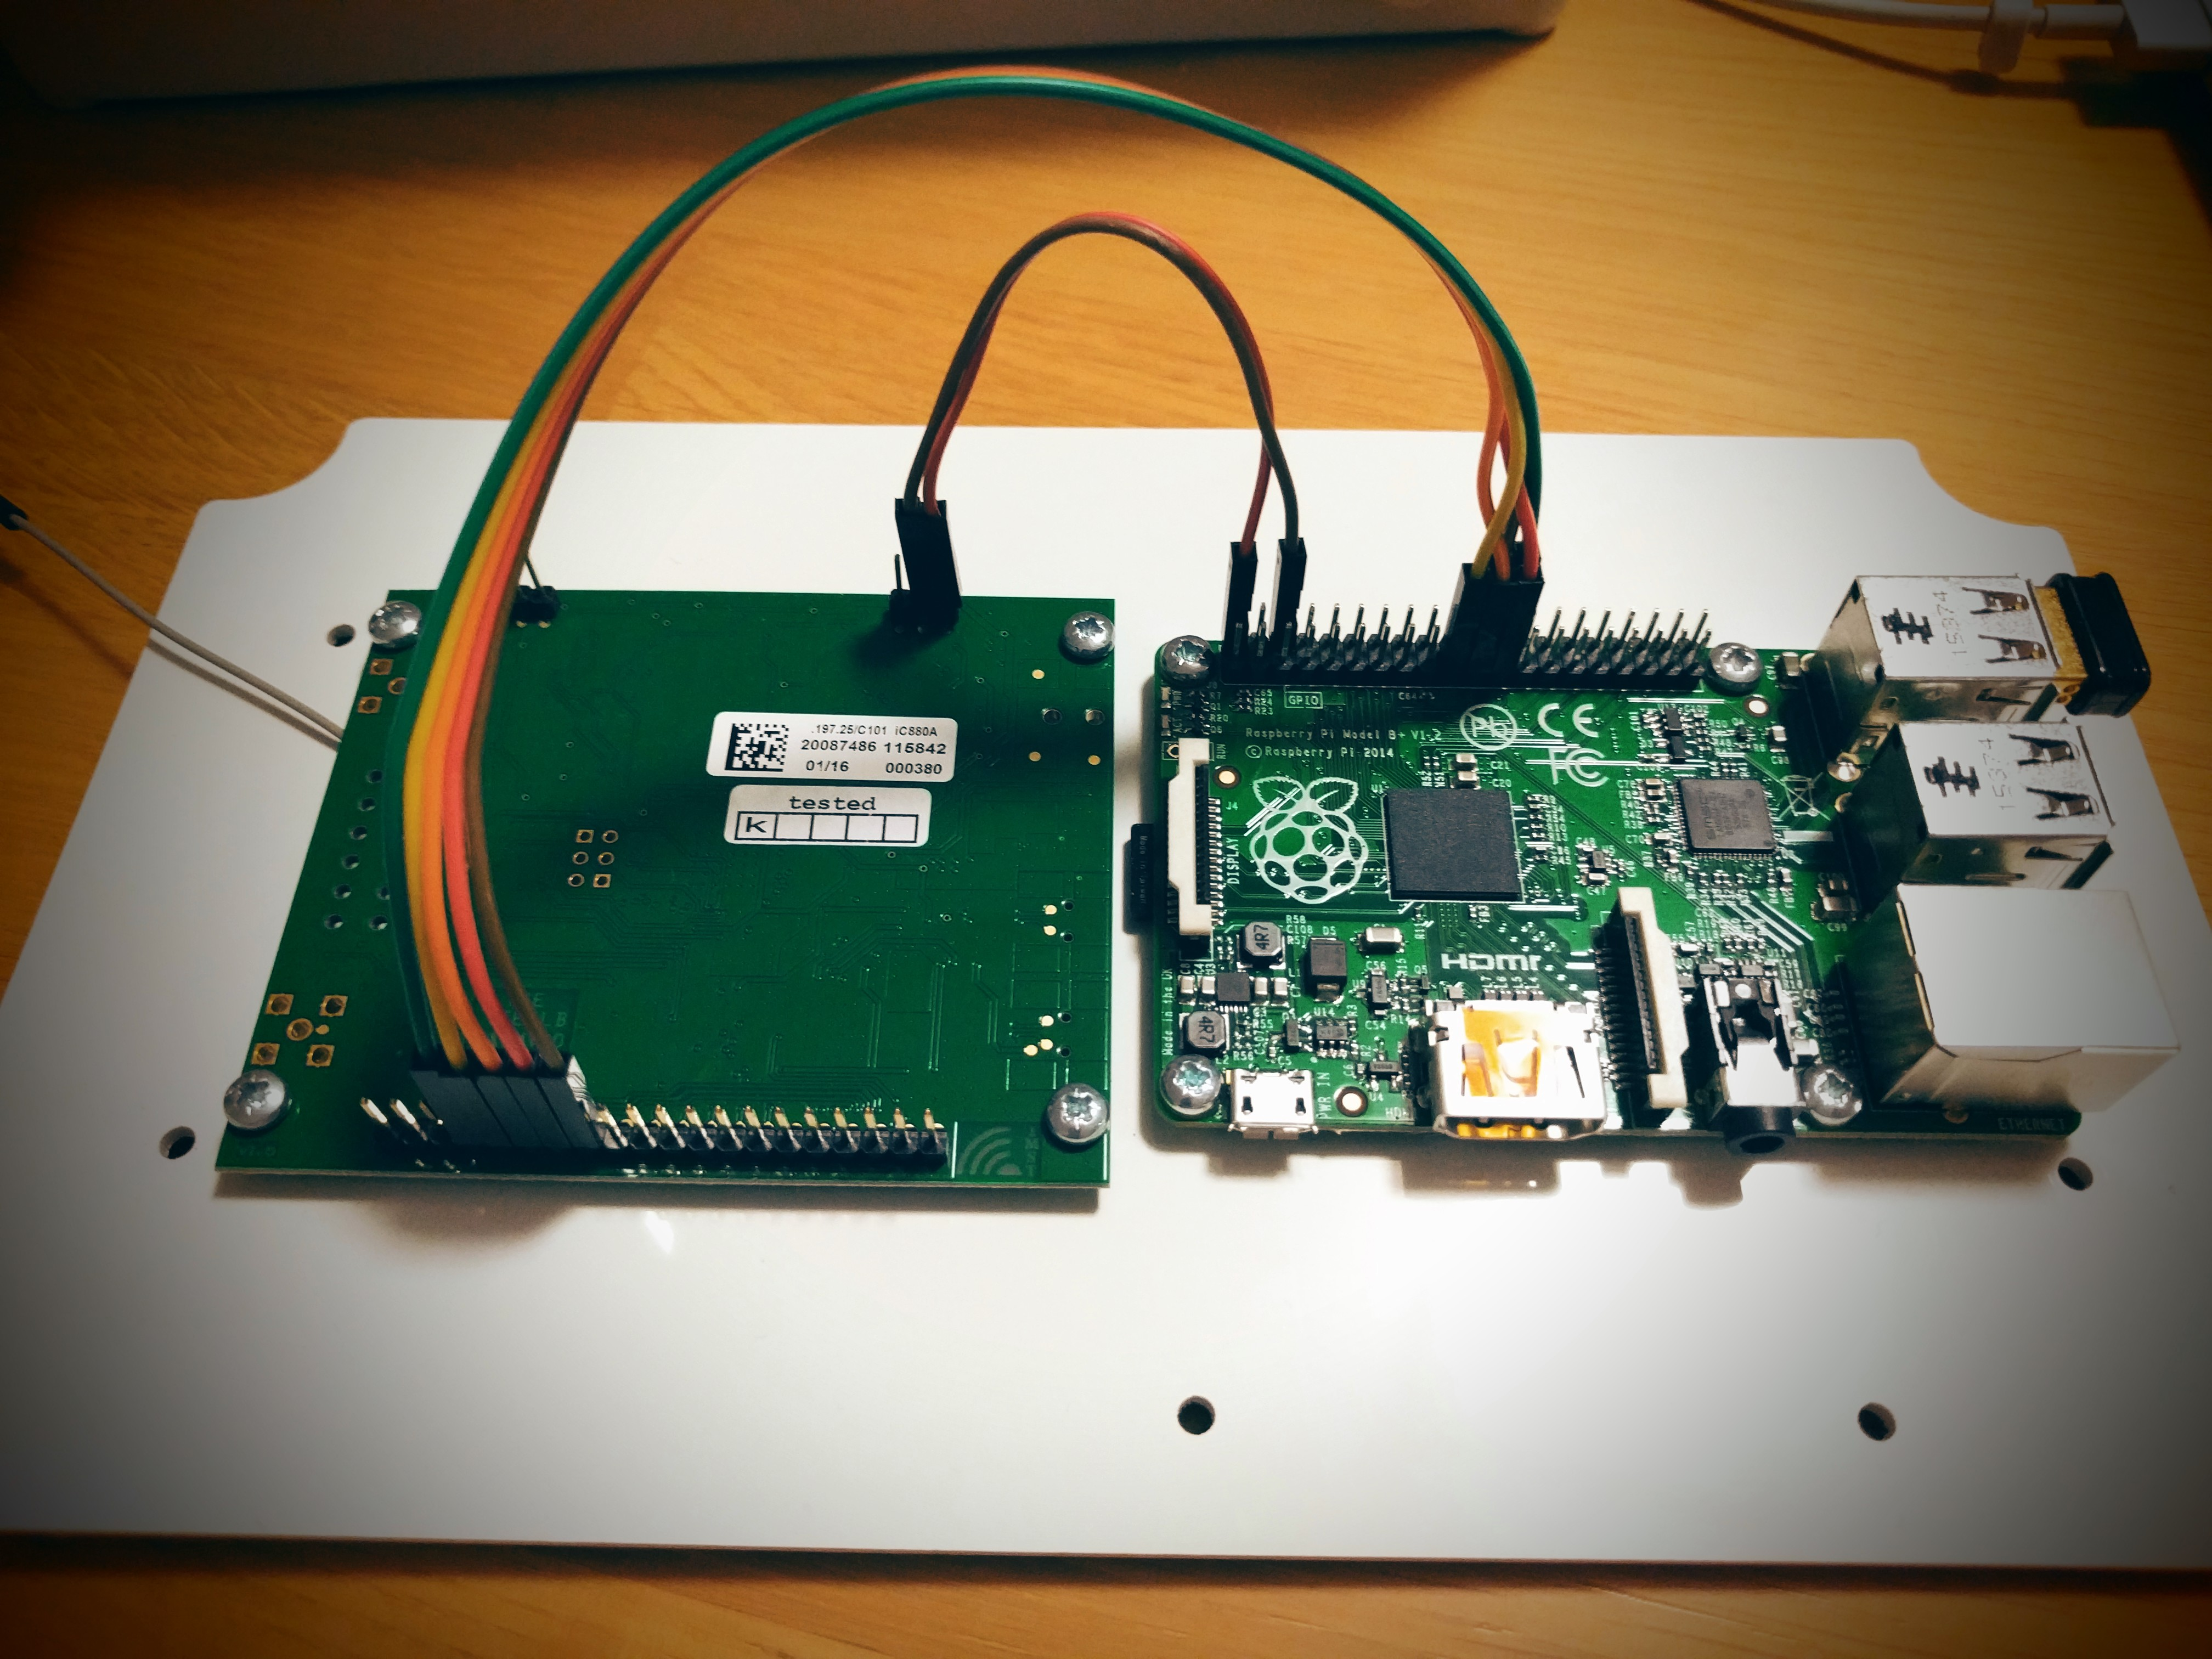
\includegraphics[width=\textwidth]{DIYloraGateway.jpg}
          \caption{DIY LoRa gateway w/ Raspberry Pi \cite{DIYLoRa}}
          \label{fig:DIY_LoRa_Gateway}
        \end{figure}
      \end{column}
    \end{columns}
  \end{frame}

  \begin{frame}{Networking}
    \frametitle{WLAN Capabilities}
    \begin{columns}
      \begin{column}{0.5\textwidth}
        \begin{itemize}
          \item 200m+ of range depending on environment
          \item Unlimited messages/day
          \item 24/7 data transmission
          \item 1840kbps+ (depending on implementation)
        \end{itemize}
      \end{column}
      \begin{column}{0.5\textwidth}
        \begin{figure}[htbp]
          \centering
          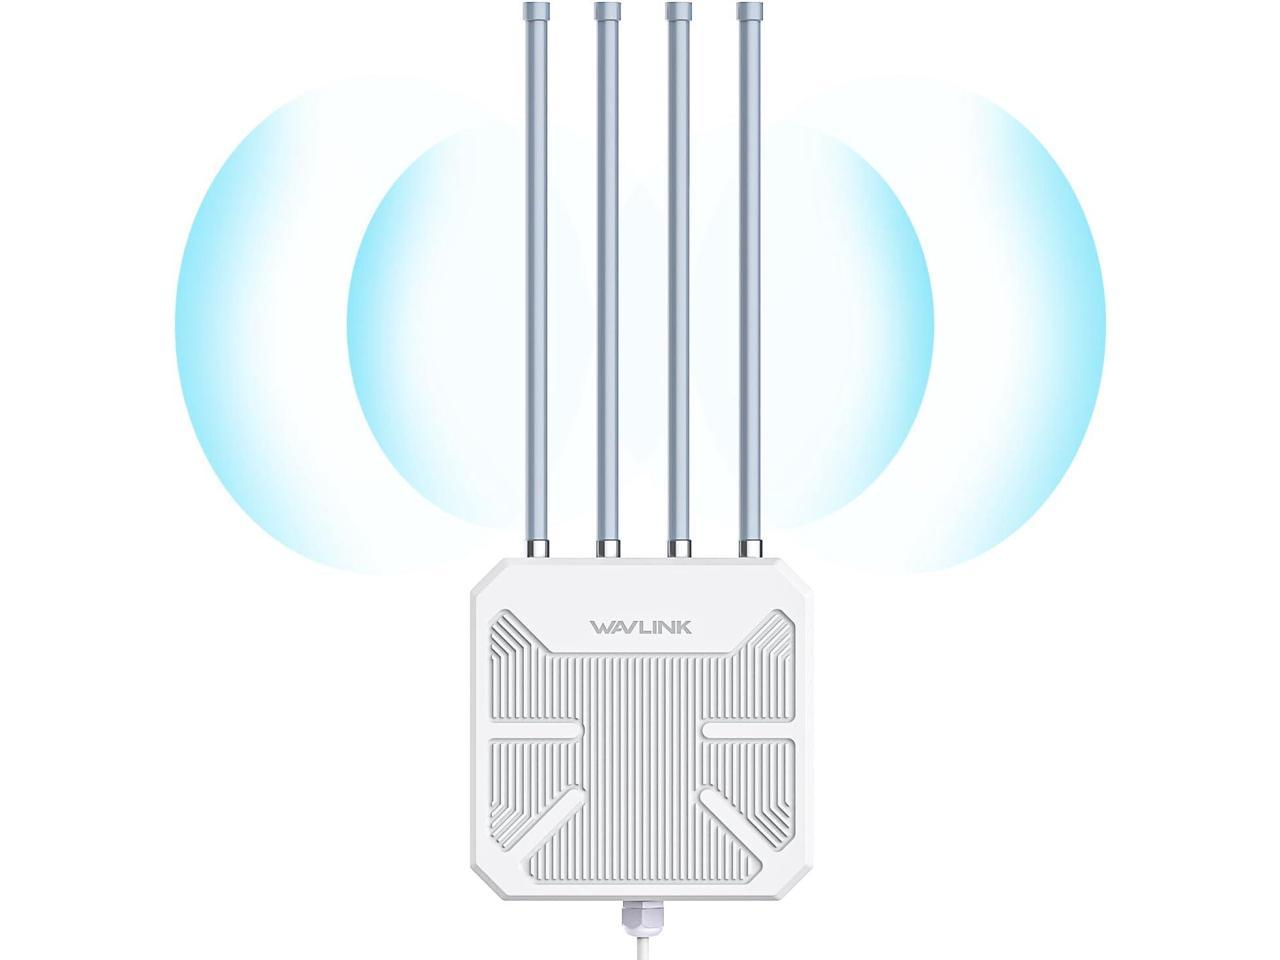
\includegraphics[width=\textwidth]{wav_link_outdoor_router.jpg}
          \caption{Wavlink AX1800 Outdoor Router}
          \label{fig:WildFi_infrastructure_overview}
        \end{figure}
      \end{column}
    \end{columns}
  \end{frame}

  \begin{frame}{Networking}
    \frametitle{WLAN Operation}
    \begin{columns}
      \begin{column}{0.5\textwidth}
        \begin{figure}[htbp]
          \centering
          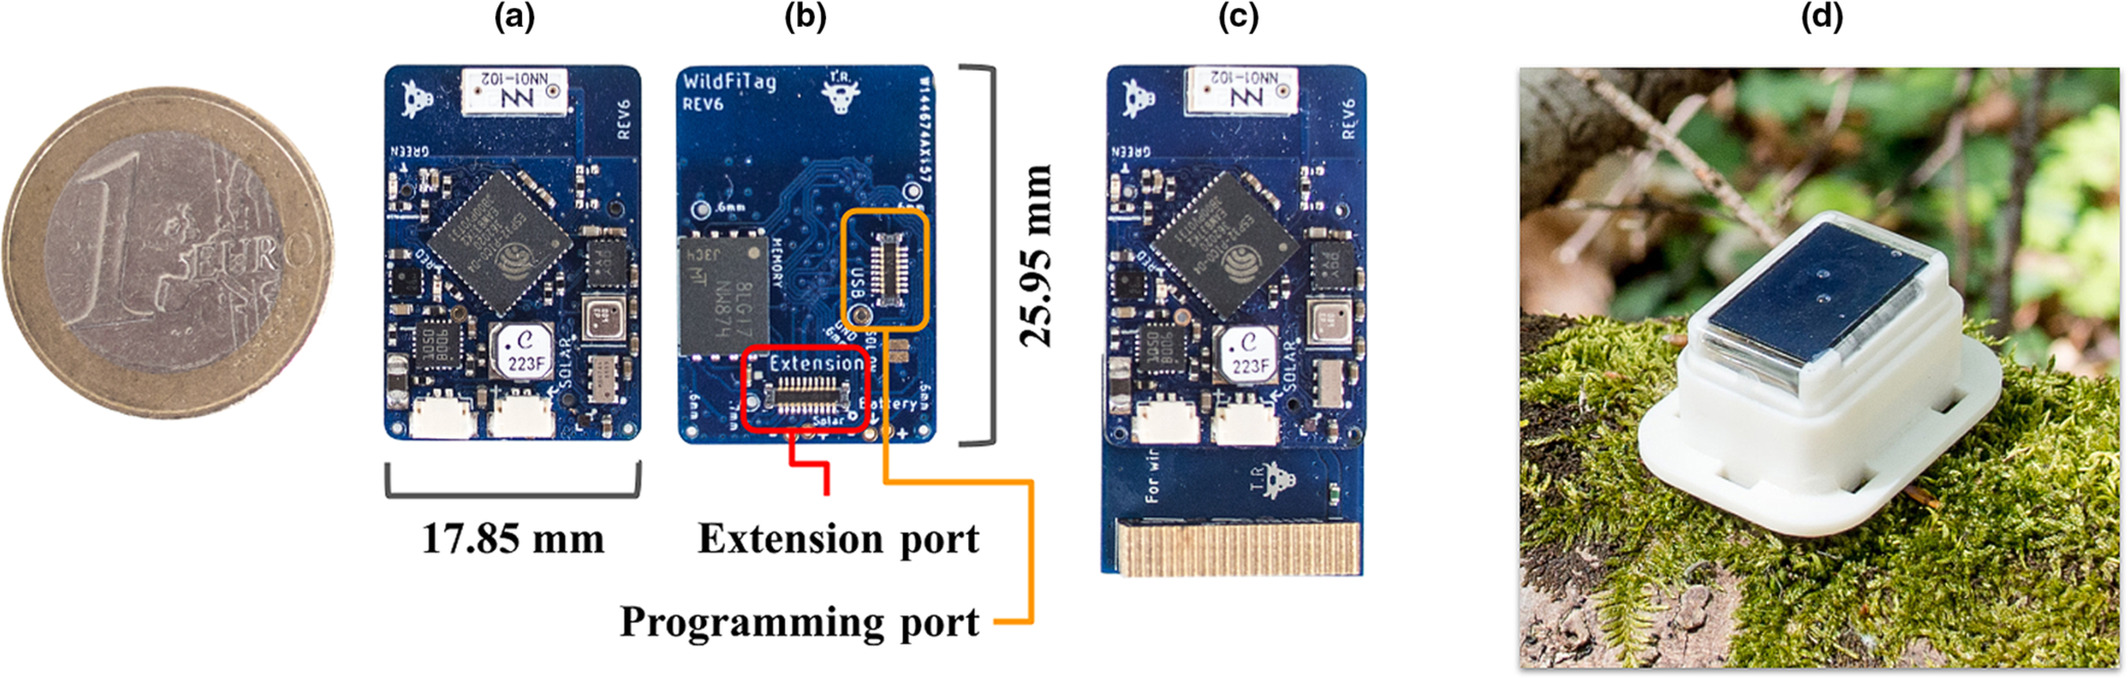
\includegraphics[width=\textwidth]{WildFi_Tag.jpg}
          \caption{WildFi tag with GPS extension and solar panel \cite{wild2023internet}}
          \label{fig:WildFi_Tag}
        \end{figure}
      \end{column}
      \begin{column}{0.5\textwidth}
        \begin{itemize}
          \item Can be entirely self developed
          \item Can last an animals lifetime with solar
          \item Cheap, Open Source, common hardware
          \item Maintained entirely by user
        \end{itemize}
      \end{column}
    \end{columns}
  \end{frame}

\subsection{Security}

\begin{frame}{Security}
  \frametitle{Security with AES-128 Encryption}
  \begin{columns}
    \begin{column}{0.5\textwidth}
      \begin{itemize}
        \item Proven track record
        \item Secures data over the air
        \item Small 128bit encryption keys
        \item Not computationally expensive
        \item \faThumbsOUp$ $ Security on battery powered devices
      \end{itemize}
    \end{column}
    \begin{column}{0.5\textwidth}
      \begin{figure}[htbp]
        \centering
        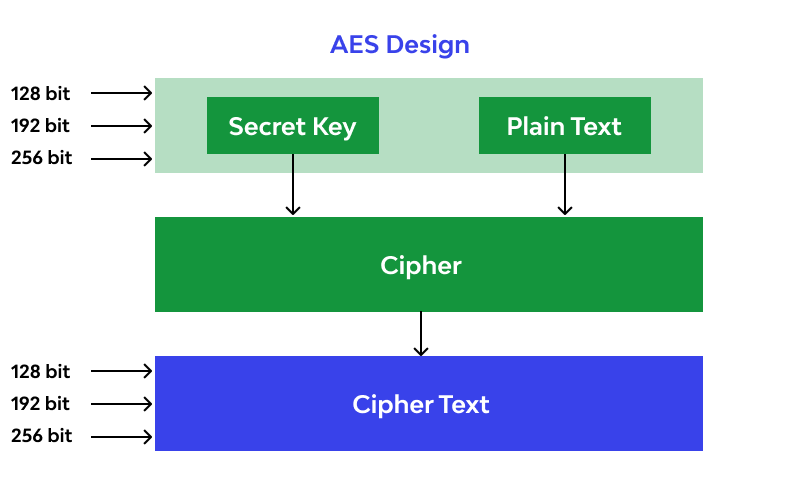
\includegraphics[width=\textwidth]{AES128_structure.png}
        \caption{AES Design \cite{Beschokov}}
        \label{fig:AES_Design}
      \end{figure}
    \end{column}
  \end{columns}
\end{frame}


  \begin{frame}{Security}
    \frametitle{SigFox, LoRa, and WLAN Security}
    \begin{columns}
      \begin{column}{0.5\textwidth}
        \begin{figure}[htbp]
          \centering
          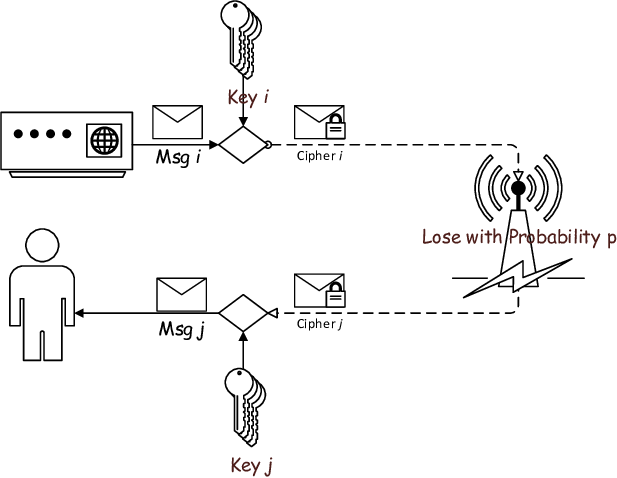
\includegraphics[width=\textwidth]{Model-of-LPWAN-Chaining-Encryption.png}
          \caption{Model of LPWAN Chaining Encryption \cite{bidgoly2019novel}}
          \label{fig:LPWAN_encryption}
        \end{figure}
      \end{column}
      \begin{column}{0.5\textwidth}
        \begin{itemize}
          \item SigFox, LoRa and WLAN can use AES-128
          \item End-to-End encryption
          \item Encrypted at the source (sensor device)
          \item Per device keys for physical protection
        \end{itemize}
      \end{column}
    \end{columns}
  \end{frame}

\subsection{Comparisons}

\begin{frame}{Comapisons}
  \frametitle{LPWAN Network Comparisons}
  \begin{columns}
    \begin{column}{0.5\textwidth}
      \begin{itemize}
        \item SigFox
        \begin{itemize}
          \item Better range and coverage
          \item Worse latency and payload
        \end{itemize}
        \item LoRa
        \begin{itemize}
          \item Easier to deploy (Private)
          \item Less data restrictions
        \end{itemize}
      \end{itemize}
    \end{column}
    \begin{column}{0.5\textwidth}
      \begin{figure}[htbp]
        \centering
        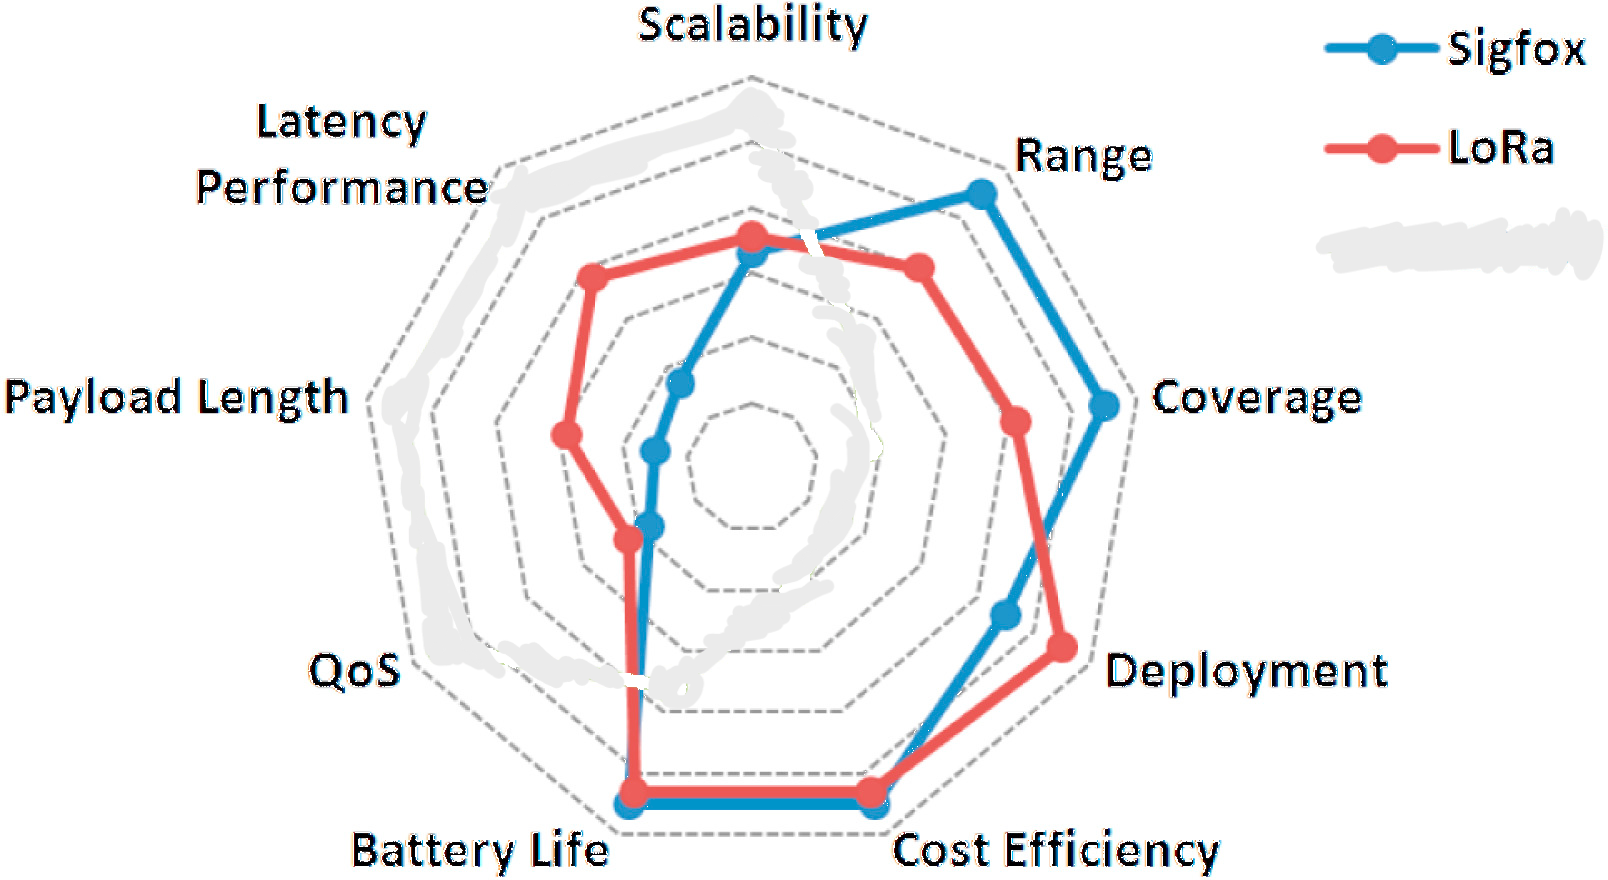
\includegraphics[width=\textwidth]{LPWAN_comparisons.png}
        \caption{LPWAN Comparisons \cite{mekki2019comparative}}
        \label{fig:LPWAN_Comparisons_map}
      \end{figure}
    \end{column}
  \end{columns}
\end{frame}

\begin{frame}{Comparisons}
  \frametitle{Final comparisons}
  \begin{columns}
    \begin{column}{\textheight}
      \begin{figure}[htbp]
        \centering
        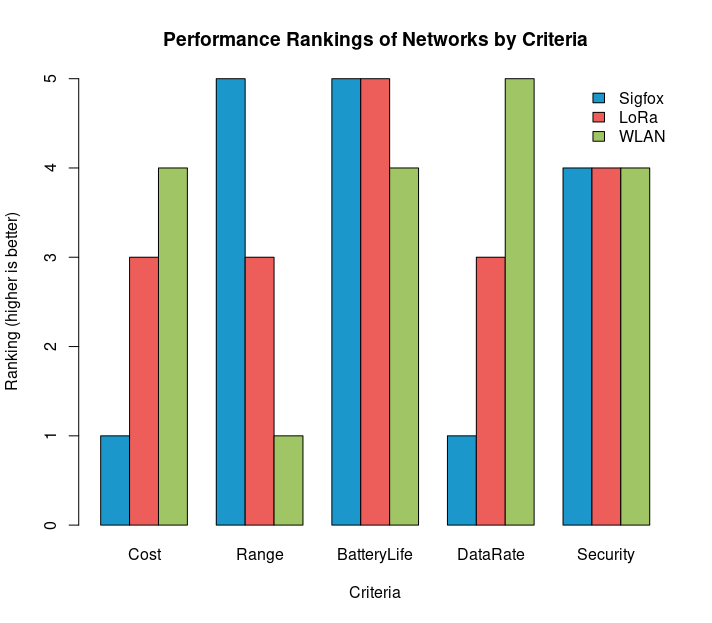
\includegraphics[width=\textwidth]{Network_Comparison_barplot.png}
        \label{fig:Network_comparison_barplot}
      \end{figure}
    \end{column}
  \end{columns}
\end{frame}

\section{Conclusion}

\begin{frame}{Conclusion}
  \frametitle{Benefits of IoT for biologging}
  \begin{columns}
    \begin{column}{0.5\textwidth}
      \begin{itemize}
        \item Bigger data payloads
        \item Highly customizable
        \item Many existing components
        \item Battery lasts for a lifetime
        \item Less disruptive tagging
      \end{itemize}
    \end{column}
    \begin{column}{0.5\textwidth}
      \begin{figure}[htbp]
        \centering
        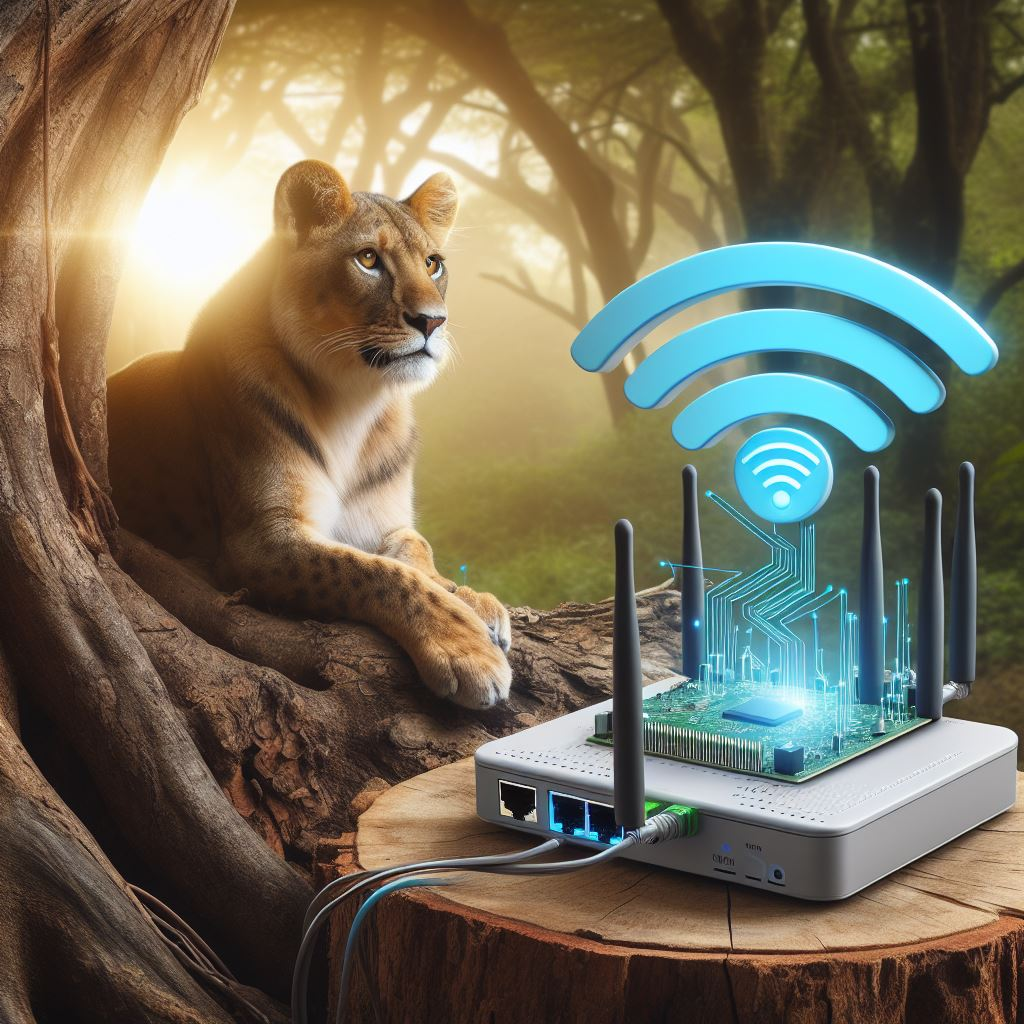
\includegraphics[width=.9\textwidth]{IoT_Lion.jpg}
        \caption{IoT sensor device on an animal in the wild [DALL$\cdot$E 3]}
        \label{fig:IoT_Lion}
      \end{figure}
    \end{column}
  \end{columns}
\end{frame}

\section{Questions}

\begin{frame}{Questions}
  \centering \Large
  \emph{Thanks for Listening!}

  Any Questions?

  \begin{figure}[htbp]
    \centering
    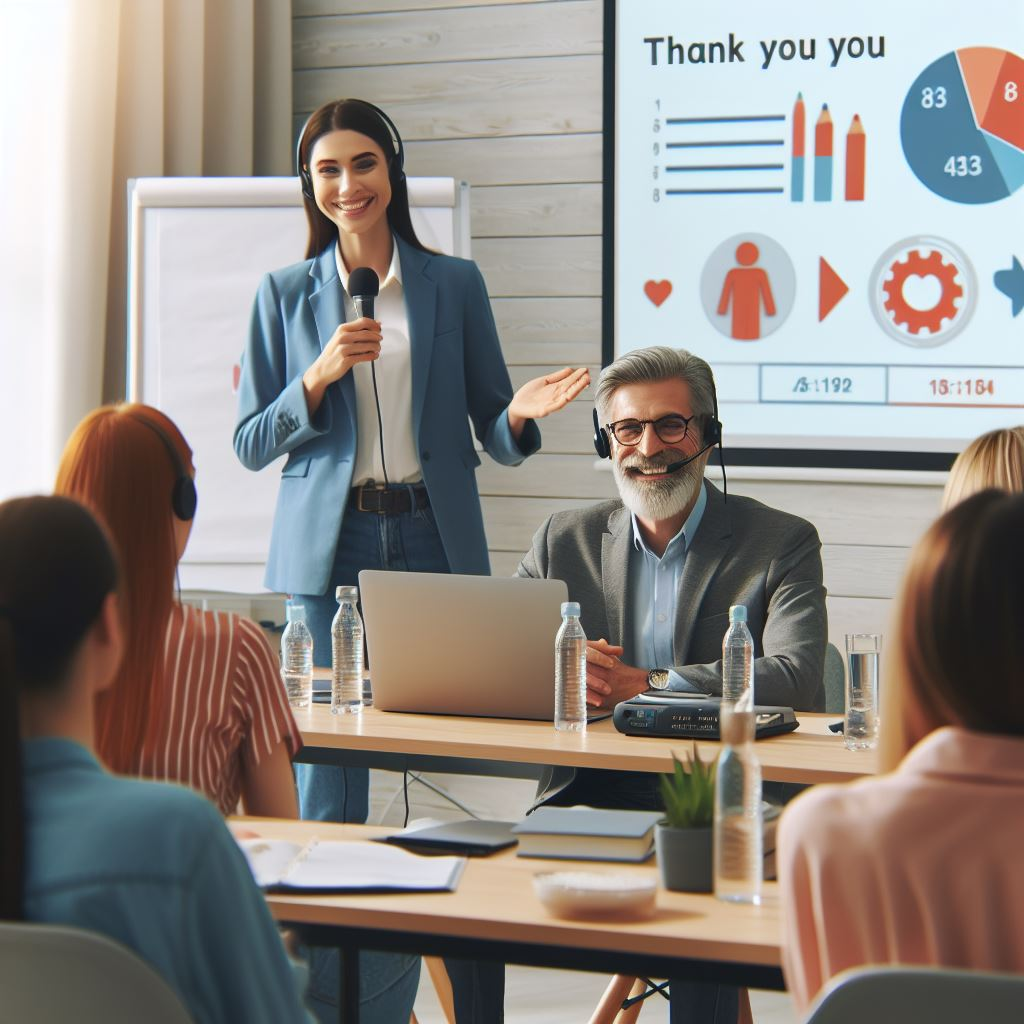
\includegraphics[height=.6\textheight]{Thank_you.jpg}
    \label{fig:Thank_you}
  \end{figure}
\end{frame}

\begin{frame}[allowframebreaks]
  \frametitle{References}
  \printbibliography
\end{frame}


\end{document}